\documentclass{article}

\usepackage{dirtree}

\usepackage[
  height=9in,      % height of the text block
  width=7.5in,       % width of the text block
  top=78pt,        % distance of the text block from the top of the page
  headheight=48pt, % height for the header block
  headsep=12pt,    % distance from the header block to the text block
  heightrounded,   % ensure an integer number of lines
        % show the main blocks
  verbose,         % show the values of the parameters in the log file
]{geometry}
\setlength{\parindent}{0pt}
\usepackage{amsmath}
\usepackage{courier}
\usepackage{graphicx}
\usepackage{amsmath}
\usepackage{booktabs}
\usepackage{fancyhdr}
\usepackage{float}
\usepackage{mathtools}

\pagestyle{fancy}
\fancyhead[L]{Pattern and Speech Recognition WS1617\\ Assignment 03}
\fancyhead[R]{ Vinh Thinh Ho (2562630) \\ Noshaba Cheema (2562653)}



\renewcommand{\headrulewidth}{0.4pt}
\newcommand\tab[1][1cm]{\hspace*{#1}}

\begin{document}
\section*{1) Linear Regression}
\subsection*{Exercise 3.1}
\subsubsection*{a, b)}
\begin{figure}[H]
	\centering
	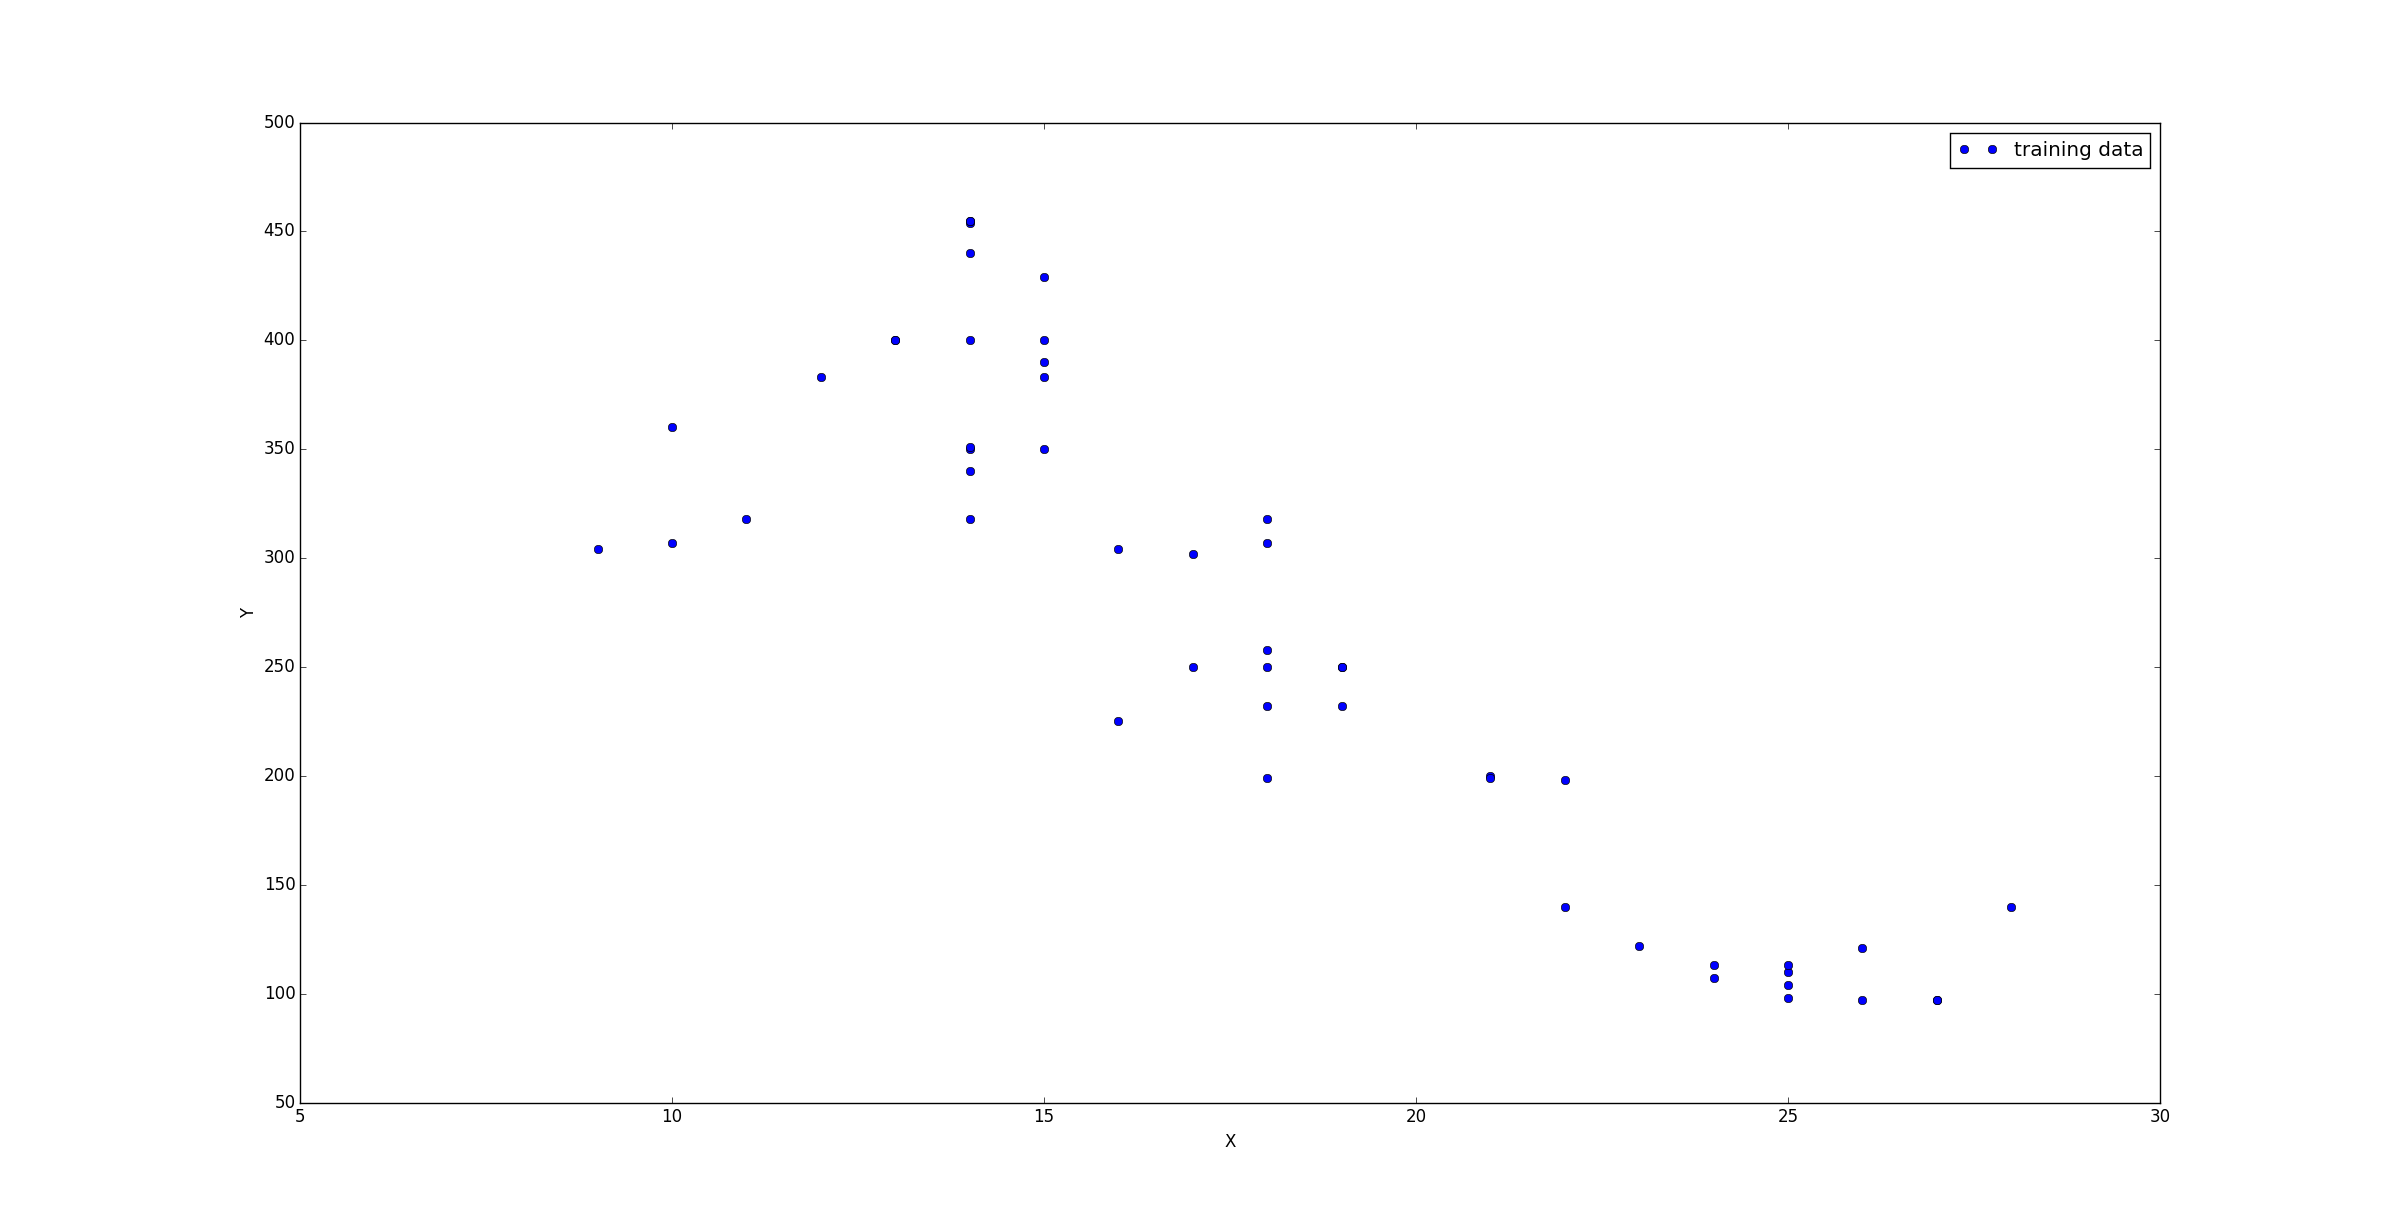
\includegraphics[scale=0.2]{31b.png}
	\caption{Training data points}
	\label{fig1}
\end{figure}

From the figure \ref{fig1}, we think that the the polynomial function that estimate these data points has degree 3, because we can see that there are 2 stationary points: 1 local maximum at \textbf{x} around [12,15] and 1 local minimum at \textbf{x} around [25,27]
\subsubsection*{c)}
With first order model, we have the equation of the polynomial model:
\begin{align*}
y = ax + b = X w
\end{align*}
Where $X$ is the Vandermonde matrix of $x$ of degree 1, meaning $X = \begin{pmatrix*}x^1 & x^0\end{pmatrix*}$ and $w$ is the weight vector with $w = \begin{pmatrix*} a \\ b \end{pmatrix*}$.\\
We use the mean square error as the loss function (we multiplied it by 0.5 so we don't have to multiply the gradient by 2.):
\begin{align*}
L = \frac{1}{2n}\sum\limits_{i=1}^{n}(y_{i} - (ax_{i} +b))^2 = \frac{1}{n}(Xw - y)^T (Xw - y)
\end{align*}
Hence, the first derivative with respect to parameter \textbf{a} and \textbf{b}:
\begin{align*}
\frac{\partial L}{\partial a} &= \frac{1}{n}\sum\limits_{i=1}^{n}-x_i(y_i - ax_i - b)\\
\frac{\partial L}{\partial b} &= \frac{1}{n}\sum\limits_{i=1}^{n}-(y_i - ax_i - b)
\end{align*}
So, we have update rule:
\begin{align*}
a_{new} &= a_{old} - \alpha\frac{\partial L}{\partial a}\\
&= a_{old} + \frac{\alpha}{n}\sum\limits_{i=1}^{n}x_i(y_i - ax_i - b)\\
b_{new} &= b_{old} - \alpha\frac{\partial L}{\partial b}\\
&= b_{old} + \frac{\alpha}{n}\sum\limits_{i=1}^{n}(y_i - ax_i - b)
\end{align*}
Or in vectorized form:\\
\begin{align*}
\frac{\partial L}{\partial w} &= \frac{1}{n} X^T(Xw - y) \\
w_{new} &= w_{old} - \alpha \frac{\partial L}{\partial w} \\
&= w_{old} - \frac{\alpha}{n} X^T(Xw - y)
\end{align*}
Where n = 50, which is the number of training data points; and $\alpha$ is learning rate.

\subsubsection*{d, e)}
We initialized the weights $w$ randomly and the learning rate as $\alpha = 0.0028$\\
We stopped at 10000 iterations as the loss did not seem to change much.\\
The parameter we found were: $w = (a, b) = (-15.74831151,  546.24744732)$.
The final mean squared error that we get is $\approx 3559.44$.
The final cost function value is $\approx 1779.72$ as we half the MSE for numerical reasons.
\begin{figure}[H]
	\centering
	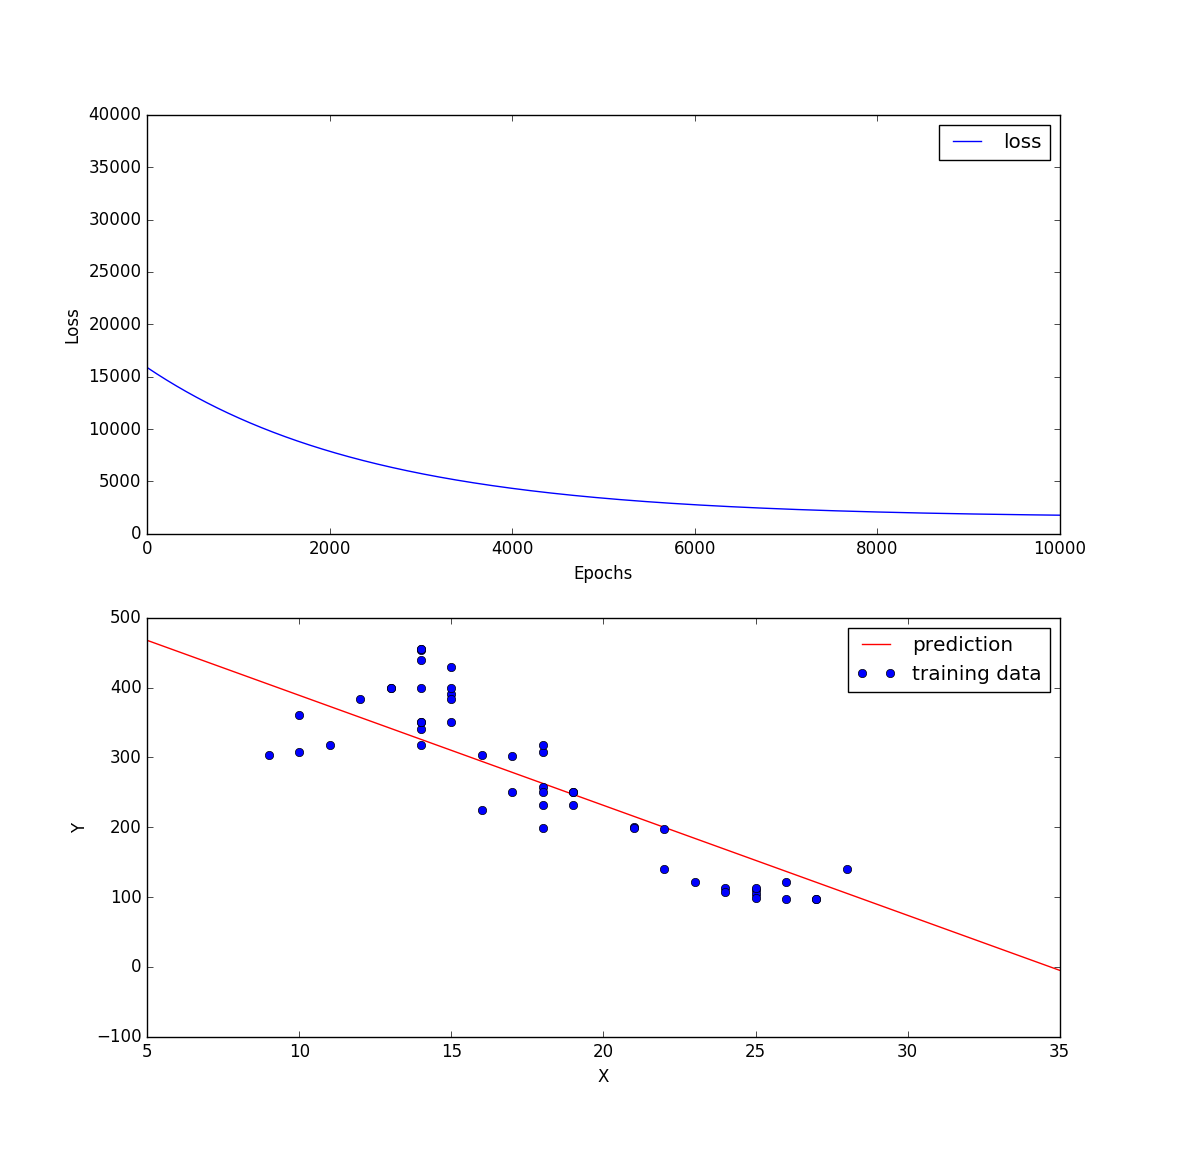
\includegraphics[scale=0.3]{31de.png}
	\caption{Loss function after each epoch of gradient descent (top) and learned first order model (bottom).}
	\label{fig2}
\end{figure}

\subsubsection*{f)}
With second order model, we have the equation of the polynomial model:
\begin{align*}
y = ax^2 + bx + c = Xw
\end{align*}
Where $X$ is the Vandermonde matrix of $x$ of degree two, meaning $X = \begin{pmatrix*}x^2 & x^1 & x^0\end{pmatrix*}$ and $w$ is the weight vector $w = \begin{pmatrix*}a \\ b \\ c\end{pmatrix*}$
We use the mean squared error multiplied by 0.5 as the loss function:
\begin{align*}
L = \frac{1}{2n}\sum\limits_{i=1}^{n}(y_{i} - (ax_{i}^2 +bx_i + c))^2 = \frac{1}{2n} (Xw - y)^T (Xw - y)
\end{align*}
Hence, the first derivatives with respect to parameters \textbf{a}, \textbf{b} and \textbf{c} are:
\begin{align*}
\frac{\partial L}{\partial a} &= \frac{1}{n}\sum\limits_{i=1}^{n}-x_i^2(y_i - ax_{i}^2 -bx_i - c)\\
\frac{\partial L}{\partial b} &= \frac{1}{n}\sum\limits_{i=1}^{n}-x_i(y_i - ax_{i}^2 -bx_i - c)\\
\frac{\partial L}{\partial c} &= \frac{1}{n}\sum\limits_{i=1}^{n}-(y_i - ax_{i}^2 -bx_i - c)
\end{align*}
or 
\begin{align*}
\frac{\partial L}{\partial w} &= \frac{1}{n} X^T(Xw - y) 
\end{align*}
So, we have update rule:
\begin{align*}
a_{new} &= a_{old} - \alpha\frac{\partial L}{\partial a}\\
&= a_{old} + \frac{\alpha}{n}\sum\limits_{i=1}^{n}x_i^2(y_i - ax_{i}^2 -bx_i - c)\\
b_{new} &= b_{old} - \alpha\frac{\partial L}{\partial b}\\
&= b_{old} + \frac{\alpha}{n}\sum\limits_{i=1}^{n}x_i(y_i - ax_{i}^2 -bx_i - c)\\
c_{new} &= c_{old} - \alpha\frac{\partial L}{\partial c}\\
&= c_{old} + \frac{\alpha}{n}\sum\limits_{i=1}^{n}(y_i - ax_{i}^2 -bx_i - c)\\
\end{align*}
Vectorized:
\begin{align*}
w_{new} &= w_{old} - \alpha \frac{\partial L}{\partial w} \\
&= w_{old} - \frac{\alpha}{n} X^T(Xw - y)
\end{align*}
Where n = 50, which is the number of training data points; and $\epsilon$ is learning rate.
\subsubsection*{g)}
We use the learning rate $\alpha$ = 0.000012 and  limit the number of epochs to 120000 and below is the loss function after each epoch and the corresponding trained model:
\begin{figure}[H]
	\centering
	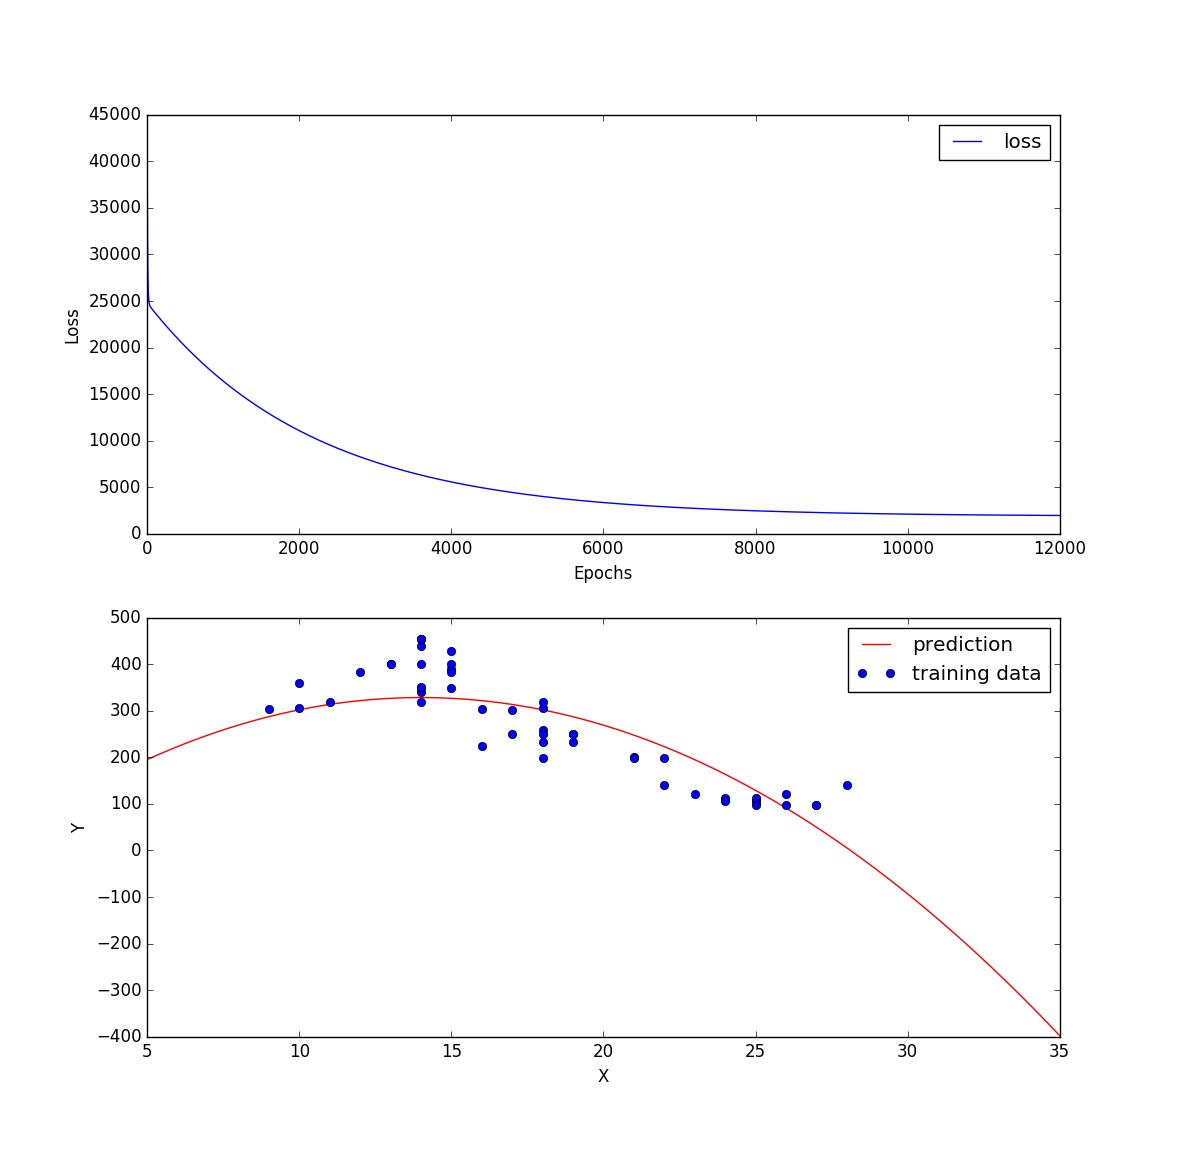
\includegraphics[scale=0.3]{31g.png}
	\caption{Loss function after each epoch in second order model (top) and learned second order model (bottom).}
	\label{fig4}
\end{figure}
Parameters found are $w = (a, b, c) = (-1.64584803,  46.06328583,   6.13825731)$ with loss value $\approx 1971.82$ and MSE $\approx 3943.64$.\\

However, this is not expected value we need, since the algorithm will continue to optimize further than 120000 epochs. We implemented the Newton method to find the expected value (see \textbf{31g\_newton.py}):
\begin{figure}[H]
	\centering
	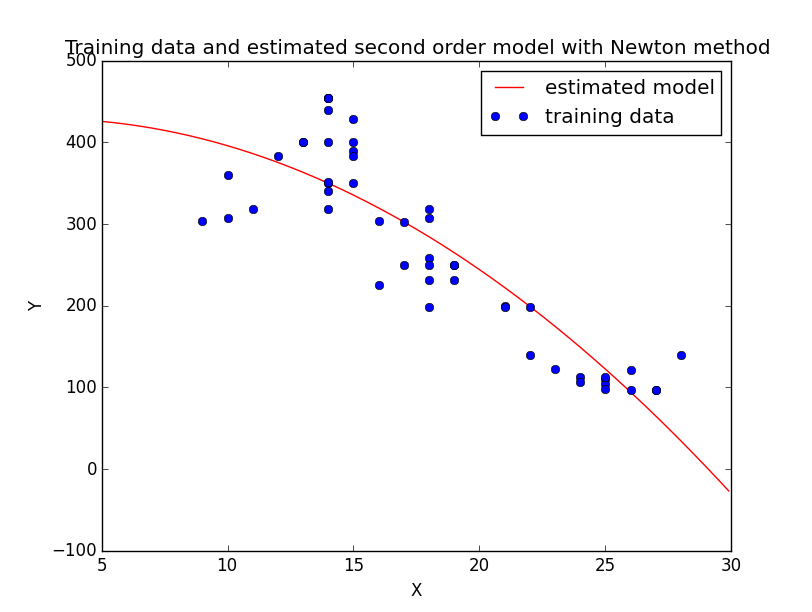
\includegraphics[scale=0.4]{31g_newton.png}
	\caption{Learned second order model with gradient descent}
	\label{fig6}
\end{figure}

The expected model is $w = (a, b, c) = (-0.613853733604, 3.249988125574, 424.868176858792)$ with MSE $\approx$ 2844.28 (see Figure \ref{fig6})

\subsection*{h)}
\begin{figure}[H]
	\centering
	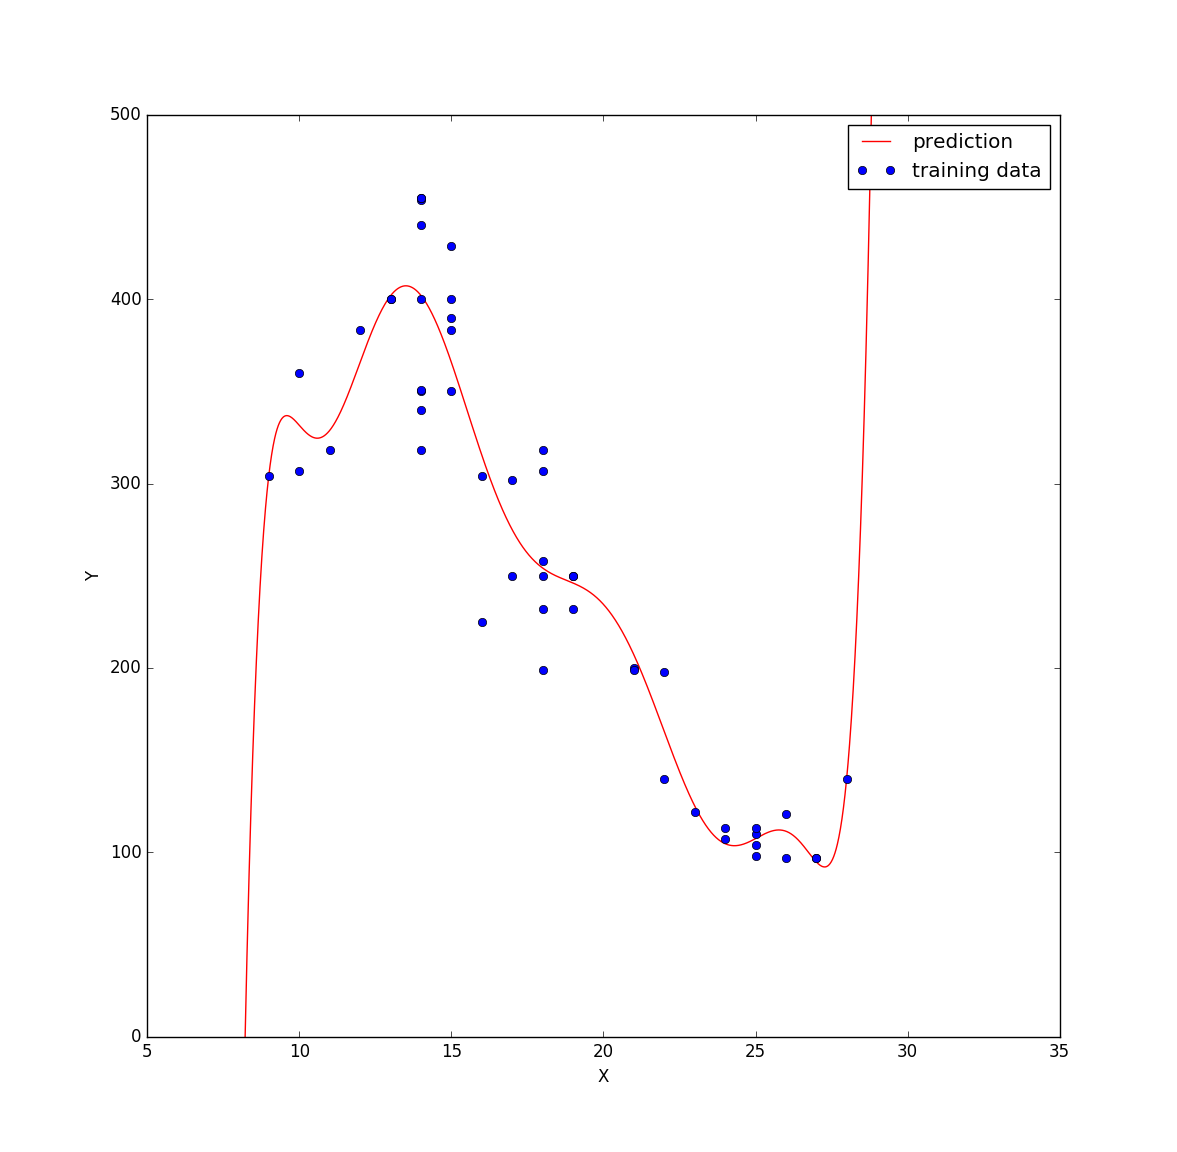
\includegraphics[scale=0.25]{31h.png}
	\caption{Training data and estimated 9th degree polynomial model}
	\label{fig7}
\end{figure}
With this model, the MSE is decreased to $\approx 1136.02$, which is better than first and second order models, however as the graph suggests, the new model looks way too overfitted.

\subsection*{i)}
\begin{figure}[H]
	\centering
	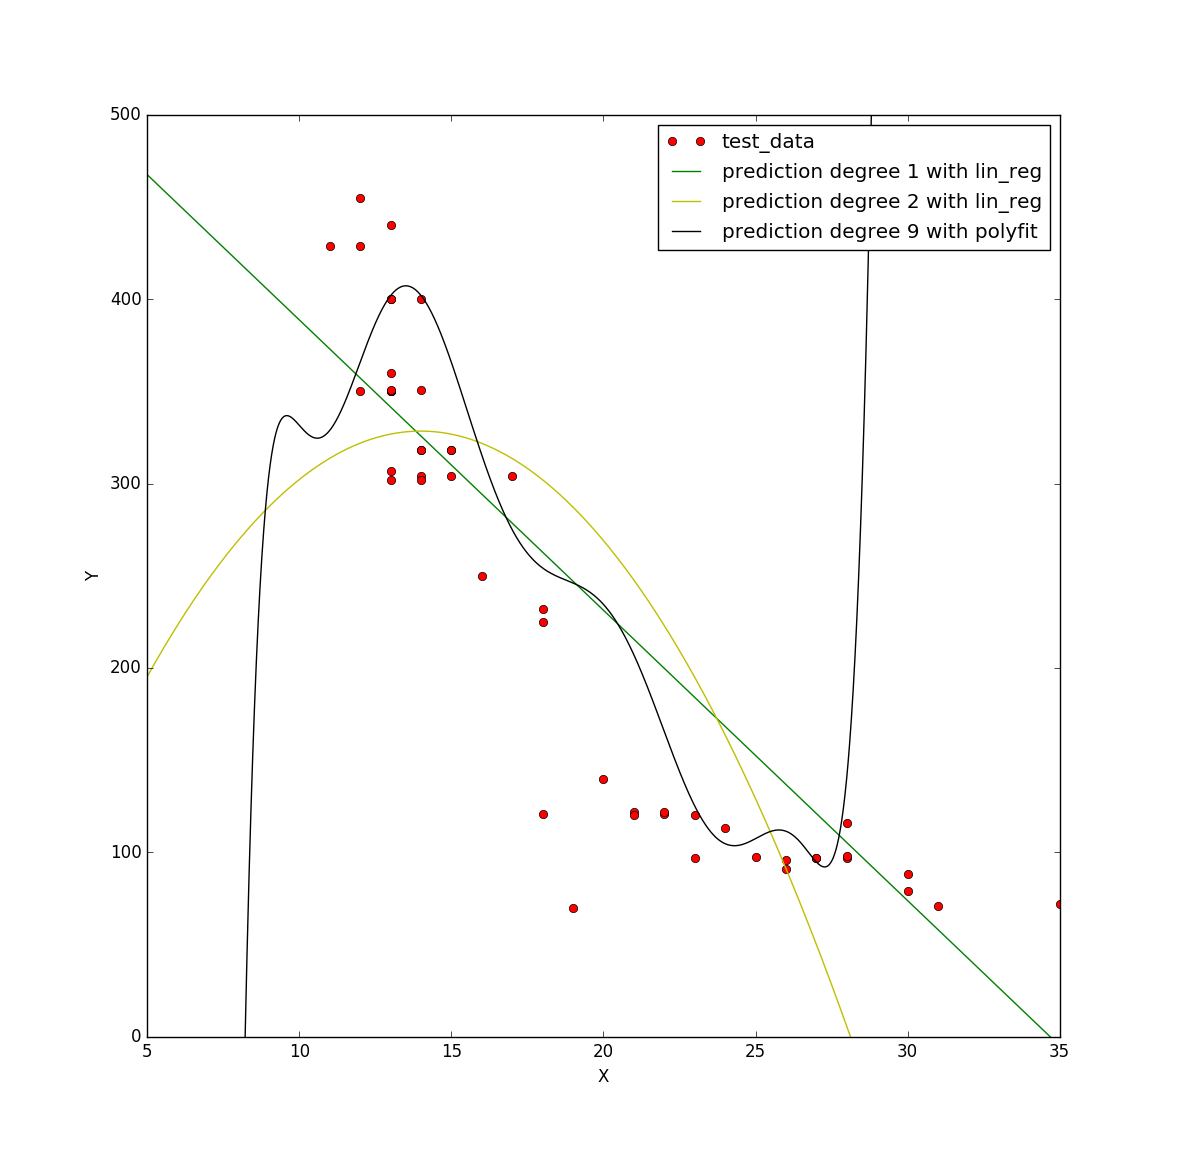
\includegraphics[scale=0.25]{31i.png}
	\caption{Test data and trained models}
	\label{fig8}
\end{figure}
MSE first order model for the test set $\approx 3389.72$\\
MSE second order model for test set $\approx 12562.16$\\
MSE 9th order model for test set $\approx 1697820189.03$\\
\\
From the Figure \ref{fig8} and the MSEs, we conclude that although the first model order fits worst for the training data, it fits best for the test data. In contrast, the ninth order model fits best for the training data, however it fits worst for the test data. Hence, the second and 9th order models are too overfitted to the training data and do not generalize well for unknown data points.
\section*{2) Regularization}
\subsection*{Exercise 3.2}
We can write the expression as:
$$J(\textbf{w}) = MSE_{train} + \lambda w^T w = \|X w - y\|^2 + \lambda w^T w = \|\tilde X w - \tilde y\|^2$$
Where $X$ is a Vandermonde matrix of the data (given an arbitrary degree) and $\tilde X= \begin{pmatrix*}X \\ \sqrt{\lambda} I\end{pmatrix*}$.\\
$y$ is the class label vector and $\tilde y = \begin{pmatrix*}y \\ 0\end{pmatrix*}$ and $w$ is the weight vector.
Since we want to minimize the expression $ \|\tilde X w - \tilde y\|^2$, we equate it to 0 and solve for $w$ to get our closed form expression:
\begin{align*}
\|\tilde X w - \tilde y\|^2 = (\tilde X w - \tilde y)^T (\tilde X w - \tilde y) &= 0\\
w^T \tilde X^T \tilde X w - 2 w^T \tilde X \tilde y + \tilde y^T \tilde y &= 0 \\
2 \tilde X^T \tilde X w - 2 \tilde X^T \tilde y &= 0 \\
w &= (\tilde X^T \tilde X)^{-1} \tilde X^T \tilde y \\
w &= (X^T X + \lambda I)^{-1} X^T y 
\end{align*}

\end{document}



